% The sum 1+2+4+8 fills every unit of a bar of length 16 except the last.
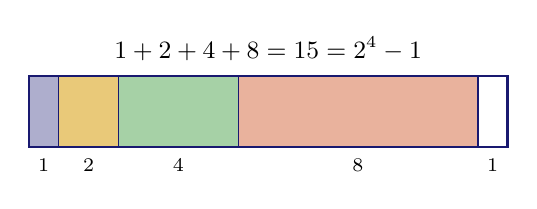
\begin{tikzpicture}[x=0.38cm,y=1cm]
  \fill[MidnightBlue!35] (0,0) rectangle (1,0.9);
  \fill[Goldenrod!60] (1,0) rectangle (3,0.9);
  \fill[ForestGreen!40] (3,0) rectangle (7,0.9);
  \fill[BrickRed!28] (7,0) rectangle (15,0.9);
  \draw[MidnightBlue,thick] (0,0) rectangle (15,0.9);
  \draw[MidnightBlue,thick] (15,0) rectangle (16,0.9);
  \draw[MidnightBlue] (1,0) -- (1,0.9);
  \draw[MidnightBlue] (3,0) -- (3,0.9);
  \draw[MidnightBlue] (7,0) -- (7,0.9);
  \node[font=\scriptsize,below=1pt] at (0.5,0) {$1$};
  \node[font=\scriptsize,below=1pt] at (2,0) {$2$};
  \node[font=\scriptsize,below=1pt] at (5,0) {$4$};
  \node[font=\scriptsize,below=1pt] at (11,0) {$8$};
  \node[font=\scriptsize,below=1pt] at (15.5,0) {$1$};
  \node[font=\small,above=2pt] at (8,0.9) {$1+2+4+8=15=2^{4}-1$};
\end{tikzpicture}
